\documentclass[12pt,a4paper]{article}
\usepackage[utf8]{inputenc}
\usepackage[margin=1in]{geometry}
\usepackage{graphicx}
\usepackage{listings}
\usepackage{xcolor}
\usepackage{amsmath}
\usepackage{fancyhdr}
\usepackage{titlesec}
\usepackage{hyperref}
\usepackage{float}

% Code listing style
\definecolor{codegreen}{rgb}{0,0.6,0}
\definecolor{codegray}{rgb}{0.5,0.5,0.5}
\definecolor{codepurple}{rgb}{0.58,0,0.82}
\definecolor{backcolour}{rgb}{0.95,0.95,0.92}

\lstdefinestyle{mystyle}{
    backgroundcolor=\color{backcolour},   
    commentstyle=\color{codegreen},
    keywordstyle=\color{magenta},
    numberstyle=\tiny\color{codegray},
    stringstyle=\color{codepurple},
    basicstyle=\ttfamily\footnotesize,
    breakatwhitespace=false,         
    breaklines=true,                 
    captionpos=b,                    
    keepspaces=true,                 
    numbers=left,                    
    numbersep=5pt,                  
    showspaces=false,                
    showstringspaces=false,
    showtabs=false,                  
    tabsize=4
}
\lstset{style=mystyle}

% Header and Footer
\pagestyle{fancy}
\fancyhf{}
\rhead{Computer Graphics Lab}
\lhead{Lab 2}
\rfoot{Page \thepage}

\begin{document}

% Title Page
\begin{titlepage}
    \centering
    \vspace*{1cm}
    
    \Huge
    \textbf{Computer Graphics Laboratory}
    
    \vspace{0.5cm}
    \LARGE
    Lab Report 2
    
    \vspace{1.5cm}
    
    \Large
    \textbf{Line Drawing, Circle, Ellipse Algorithms \& Chart Implementation}
    
    \vspace{2cm}
    
    \textbf{Submitted By:}\\
    \vspace{0.3cm}
    \Large
    Utsav Adhikari
    
    \vspace{2cm}
    
    \textbf{Date:}\\
    \vspace{0.3cm}
    \today
    
    \vfill
    
    \large
    Department of Computer Science\\
    5th Semester
    
\end{titlepage}

\tableofcontents
\newpage

%===========================================
% TASK 1: DDA LINE DRAWING ALGORITHM
%===========================================
\section{Digital Differential Analyzer (DDA) Line Drawing Algorithm}

\subsection{Title of Lab Activity}
Implementation of Digital Differential Analyzer (DDA) algorithm for drawing a straight line between two given endpoints.

\subsection{Algorithm}
The DDA algorithm is an incremental scan conversion method that calculates intermediate points along a line path by using the line equation.

\textbf{Steps:}
\begin{enumerate}
    \item Input the two endpoints of the line: $(x_0, y_0)$ and $(x_1, y_1)$
    \item Calculate $dx = x_1 - x_0$ and $dy = y_1 - y_0$
    \item Calculate the number of steps: $steps = \max(|dx|, |dy|)$
    \item Calculate increments: $x_{inc} = \frac{dx}{steps}$ and $y_{inc} = \frac{dy}{steps}$
    \item Initialize starting point: $x = x_0$, $y = y_0$
    \item For $i = 0$ to $steps$:
    \begin{itemize}
        \item Plot pixel at $(\text{round}(x), \text{round}(y))$
        \item Update: $x = x + x_{inc}$, $y = y + y_{inc}$
    \end{itemize}
\end{enumerate}

\subsection{Source Code}
\begin{lstlisting}[language=Python, caption=DDA Line Drawing Algorithm]
def dda_line(surface, x0, y0, x1, y1, color):
    """
    Digital Differential Analyzer Line Drawing Algorithm
    Draws a line from (x0, y0) to (x1, y1)
    """
    dx = x1 - x0
    dy = y1 - y0
    
    # Calculate number of steps required
    steps = int(max(abs(dx), abs(dy)))
    
    if steps == 0:
        plot(surface, x0, y0, color)
        return
    
    # Calculate increment for each step
    x_inc = dx / steps
    y_inc = dy / steps
    
    x = x0
    y = y0
    
    # Plot pixels along the line
    for _ in range(steps + 1):
        plot(surface, int(round(x)), int(round(y)), color)
        x += x_inc
        y += y_inc
\end{lstlisting}

\subsection{Output}
\begin{figure}[H]
    \centering
    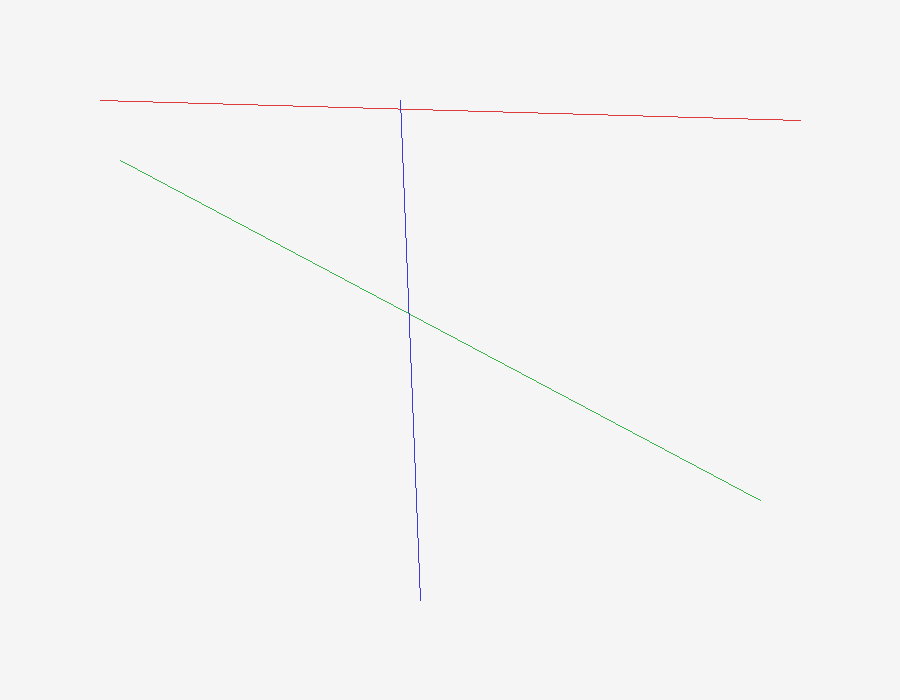
\includegraphics[width=0.8\textwidth]{out_1_dda_lines.png}
    \caption{DDA Line Drawing Algorithm Output}
\end{figure}

\newpage
%===========================================
% TASK 2: BRESENHAM LINE DRAWING ALGORITHM
%===========================================
\section{Bresenham Line Drawing Algorithm}

\subsection{Title of Lab Activity}
Implementation of Bresenham's Line Drawing Algorithm for both slopes: $|m| < 1$ and $|m| \geq 1$.

\subsection{Algorithm}
Bresenham's algorithm uses only integer arithmetic, making it faster than DDA. It uses a decision parameter to determine the next pixel.

\subsubsection{Case 1: When $|m| < 1$ (Low Slope)}
\textbf{Steps:}
\begin{enumerate}
    \item Input endpoints $(x_0, y_0)$ and $(x_1, y_1)$
    \item Calculate $dx = |x_1 - x_0|$ and $dy = |y_1 - y_0|$
    \item Initialize decision parameter: $d = 2 \cdot dy - dx$
    \item Plot starting pixel $(x_0, y_0)$
    \item For each $x$ from $x_0$ to $x_1$:
    \begin{itemize}
        \item If $d > 0$: increment $y$, update $d = d - 2 \cdot dx$
        \item Update $d = d + 2 \cdot dy$
        \item Plot pixel $(x, y)$
    \end{itemize}
\end{enumerate}

\subsubsection{Case 2: When $|m| \geq 1$ (High Slope)}
\textbf{Steps:}
\begin{enumerate}
    \item Input endpoints $(x_0, y_0)$ and $(x_1, y_1)$
    \item Calculate $dx = |x_1 - x_0|$ and $dy = |y_1 - y_0|$
    \item Initialize decision parameter: $d = 2 \cdot dx - dy$
    \item Plot starting pixel $(x_0, y_0)$
    \item For each $y$ from $y_0$ to $y_1$:
    \begin{itemize}
        \item If $d > 0$: increment $x$, update $d = d - 2 \cdot dy$
        \item Update $d = d + 2 \cdot dx$
        \item Plot pixel $(x, y)$
    \end{itemize}
\end{enumerate}

\subsection{Source Code}
\begin{lstlisting}[language=Python, caption=Bresenham Line Drawing for $|m| < 1$]
def bresenham_line_low(surface, x0, y0, x1, y1, color):
    """
    Bresenham Line Drawing for |m| < 1 (steps in x direction)
    """
    dx = x1 - x0
    dy = y1 - y0
    xi = 1
    if dx < 0:
        xi = -1
        dx = -dx
    
    d = 2 * abs(dy) - dx
    y_step = 1 if dy >= 0 else -1
    y = y0
    x = x0
    
    for _ in range(dx + 1):
        plot(surface, x, y, color)
        if d > 0:
            y += y_step
            d -= 2 * dx
        d += 2 * abs(dy)
        x += xi
\end{lstlisting}

\begin{lstlisting}[language=Python, caption=Bresenham Line Drawing for $|m| \geq 1$]
def bresenham_line_high(surface, x0, y0, x1, y1, color):
    """
    Bresenham Line Drawing for |m| >= 1 (steps in y direction)
    """
    dx = x1 - x0
    dy = y1 - y0
    yi = 1
    if dy < 0:
        yi = -1
        dy = -dy
    
    d = 2 * abs(dx) - dy
    x_step = 1 if dx >= 0 else -1
    x = x0
    y = y0
    
    for _ in range(dy + 1):
        plot(surface, x, y, color)
        if d > 0:
            x += x_step
            d -= 2 * dy
        d += 2 * abs(dx)
        y += yi
\end{lstlisting}

\begin{lstlisting}[language=Python, caption=General Bresenham Line (Auto-selects based on slope)]
def bresenham_line(surface, x0, y0, x1, y1, color):
    """
    General Bresenham - routes to appropriate function based on slope
    """
    if x0 == x1:
        # Vertical line
        y_start, y_end = (y0, y1) if y0 <= y1 else (y1, y0)
        for y in range(y_start, y_end + 1):
            plot(surface, x0, y, color)
        return
    
    m = (y1 - y0) / (x1 - x0)
    if abs(m) < 1:
        bresenham_line_low(surface, x0, y0, x1, y1, color)
    else:
        bresenham_line_high(surface, x0, y0, x1, y1, color)
\end{lstlisting}

\subsection{Output}
\begin{figure}[H]
    \centering
    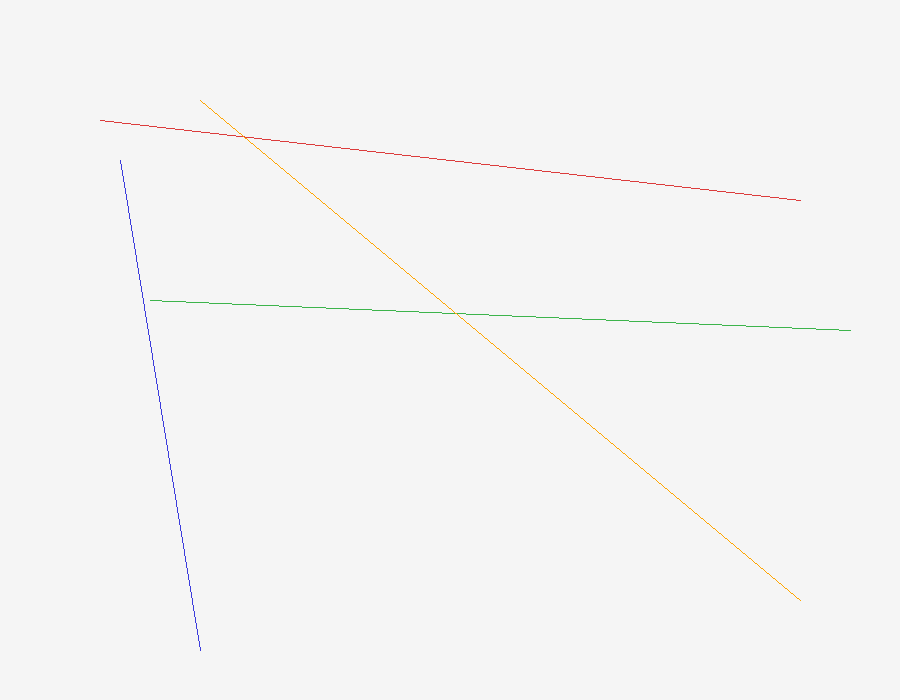
\includegraphics[width=0.8\textwidth]{out_2_bresenham_lines.png}
    \caption{Bresenham Line Drawing Algorithm Output}
\end{figure}

\newpage
%===========================================
% TASK 3: MIDPOINT CIRCLE DRAWING ALGORITHM
%===========================================
\section{Midpoint Circle Drawing Algorithm}

\subsection{Title of Lab Activity}
Implementation of Midpoint Circle Drawing Algorithm to draw a circle given center coordinates and radius.

\subsection{Algorithm}
The Midpoint Circle algorithm uses the implicit equation of a circle and exploits 8-way symmetry.

\textbf{Circle Equation:} $f(x, y) = x^2 + y^2 - r^2 = 0$

\textbf{Steps:}
\begin{enumerate}
    \item Input center $(x_c, y_c)$ and radius $r$
    \item Initialize: $x = 0$, $y = r$
    \item Calculate initial decision parameter: $d = 1 - r$
    \item Plot initial points using 8-way symmetry
    \item While $x < y$:
    \begin{itemize}
        \item If $d < 0$: $d = d + 2x + 3$
        \item Else: $d = d + 2(x - y) + 5$, decrement $y$
        \item Increment $x$
        \item Plot 8 symmetric points
    \end{itemize}
\end{enumerate}

\textbf{8-Way Symmetry Points:}
$(x_c \pm x, y_c \pm y)$ and $(x_c \pm y, y_c \pm x)$

\subsection{Source Code}
\begin{lstlisting}[language=Python, caption=Midpoint Circle Drawing Algorithm]
def _circle_symmetry(surface, xc, yc, x, y, color):
    """Plot 8 symmetric points of a circle"""
    plot(surface, xc + x, yc + y, color)
    plot(surface, xc - x, yc + y, color)
    plot(surface, xc + x, yc - y, color)
    plot(surface, xc - x, yc - y, color)
    plot(surface, xc + y, yc + x, color)
    plot(surface, xc - y, yc + x, color)
    plot(surface, xc + y, yc - x, color)
    plot(surface, xc - y, yc - x, color)


def midpoint_circle(surface, xc, yc, r, color):
    """
    Midpoint Circle Drawing Algorithm
    Draws a circle with center (xc, yc) and radius r
    """
    x = 0
    y = r
    d = 1 - r  # Initial decision parameter
    
    _circle_symmetry(surface, xc, yc, x, y, color)
    
    while x < y:
        if d < 0:
            # Select E (East)
            d = d + 2 * x + 3
        else:
            # Select SE (South-East)
            d = d + 2 * (x - y) + 5
            y -= 1
        x += 1
        _circle_symmetry(surface, xc, yc, x, y, color)
\end{lstlisting}

\subsection{Output}
\begin{figure}[H]
    \centering
    
\includegraphics[width=0.8\textwidth]{out_3_circles.png}
    \caption{Midpoint Circle Drawing Algorithm Output}
\end{figure}

\newpage
%===========================================
% TASK 4: MIDPOINT ELLIPSE DRAWING ALGORITHM
%===========================================
\section{Midpoint Ellipse Drawing Algorithm}

\subsection{Title of Lab Activity}
Implementation of Midpoint Ellipse Drawing Algorithm to draw an ellipse with given center and radii.

\subsection{Algorithm}
The algorithm divides the ellipse into two regions based on the slope and uses 4-way symmetry.

\textbf{Ellipse Equation:} $f(x, y) = r_y^2 x^2 + r_x^2 y^2 - r_x^2 r_y^2 = 0$

\textbf{Region 1:} Slope $|m| < 1$ (steps in x)
\begin{enumerate}
    \item Initialize: $x = 0$, $y = r_y$
    \item $d_1 = r_y^2 - r_x^2 r_y + 0.25 r_x^2$
    \item While $2 r_y^2 x < 2 r_x^2 y$:
    \begin{itemize}
        \item Plot 4 symmetric points
        \item If $d_1 < 0$: $d_1 = d_1 + 2 r_y^2 x + r_y^2$
        \item Else: $d_1 = d_1 + 2 r_y^2 x - 2 r_x^2 y + r_y^2$, decrement $y$
        \item Increment $x$
    \end{itemize}
\end{enumerate}

\textbf{Region 2:} Slope $|m| \geq 1$ (steps in y)
\begin{enumerate}
    \item Calculate $d_2 = r_y^2(x + 0.5)^2 + r_x^2(y - 1)^2 - r_x^2 r_y^2$
    \item While $y \geq 0$:
    \begin{itemize}
        \item Plot 4 symmetric points
        \item If $d_2 > 0$: $d_2 = d_2 + r_x^2 - 2 r_x^2 y$
        \item Else: $d_2 = d_2 + 2 r_y^2 x - 2 r_x^2 y + r_x^2$, increment $x$
        \item Decrement $y$
    \end{itemize}
\end{enumerate}

\subsection{Source Code}
\begin{lstlisting}[language=Python, caption=Midpoint Ellipse Drawing Algorithm]
def _ellipse_symmetry(surface, xc, yc, x, y, color):
    """Plot 4 symmetric points of an ellipse"""
    plot(surface, xc + x, yc + y, color)
    plot(surface, xc - x, yc + y, color)
    plot(surface, xc + x, yc - y, color)
    plot(surface, xc - x, yc - y, color)


def midpoint_ellipse(surface, xc, yc, rx, ry, color):
    """
    Midpoint Ellipse Drawing Algorithm
    Draws ellipse with center (xc, yc), x-radius rx, y-radius ry
    """
    # Region 1
    x = 0
    y = ry
    rx2 = rx * rx
    ry2 = ry * ry
    dx = 2 * ry2 * x
    dy = 2 * rx2 * y
    d1 = ry2 - rx2 * ry + 0.25 * rx2
    
    _ellipse_symmetry(surface, xc, yc, x, y, color)
    
    while dx < dy:
        if d1 < 0:
            x += 1
            dx += 2 * ry2
            d1 += dx + ry2
        else:
            x += 1
            y -= 1
            dx += 2 * ry2
            dy -= 2 * rx2
            d1 += dx - dy + ry2
        _ellipse_symmetry(surface, xc, yc, x, y, color)

    # Region 2
    d2 = ry2 * ((x + 0.5) ** 2) + rx2 * ((y - 1) ** 2) - rx2 * ry2
    
    while y >= 0:
        _ellipse_symmetry(surface, xc, yc, x, y, color)
        if d2 > 0:
            y -= 1
            dy -= 2 * rx2
            d2 += rx2 - dy
        else:
            y -= 1
            x += 1
            dx += 2 * ry2
            dy -= 2 * rx2
            d2 += dx - dy + rx2
\end{lstlisting}

\subsection{Output}
\begin{figure}[H]
    \centering
    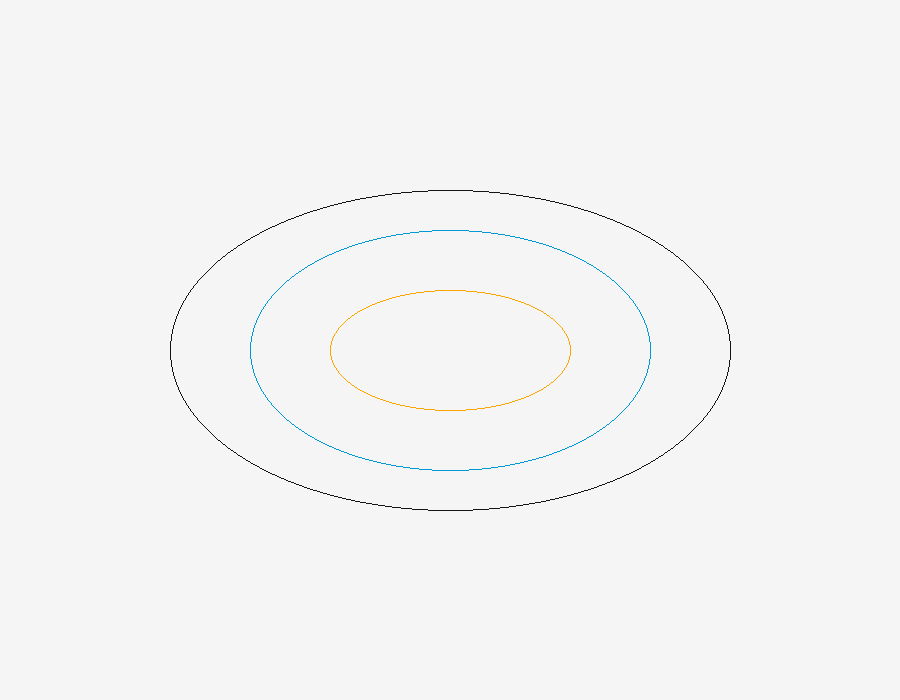
\includegraphics[width=0.8\textwidth]{out_4_ellipses.png}
    \caption{Midpoint Ellipse Drawing Algorithm Output}
\end{figure}

\newpage
%===========================================
% TASK 5: LINE GRAPH IMPLEMENTATION
%===========================================
\section{Line Graph Implementation using Line Algorithms}

\subsection{Title of Lab Activity}
Implementation of Line Graph visualization using DDA and Bresenham Line Drawing Algorithms for plotting data points.

\subsection{Algorithm}
\begin{enumerate}
    \item Input dataset as a list of values
    \item Determine the drawing area (bounding rectangle)
    \item Normalize data points to fit within the drawing area
    \item For each consecutive pair of data points:
    \begin{itemize}
        \item Convert data coordinates to screen coordinates
        \item Draw line segment using DDA or Bresenham algorithm
    \end{itemize}
    \item Draw axes for reference
\end{enumerate}

\subsection{Source Code}
\begin{lstlisting}[language=Python, caption=Line Graph Implementation]
def line_graph(surface, data, rect, color, algo='dda'):
    """
    Draw a line graph using DDA or Bresenham algorithm
    data: list of y-values
    rect: (x, y, width, height) - drawing area
    algo: 'dda' or 'bresenham'
    """
    if not data:
        return
    
    x0, y0, w, h = rect
    n = len(data)
    min_val = min(data)
    max_val = max(data)
    span = max(max_val - min_val, 1e-6)

    def to_point(i, v):
        """Convert data index and value to screen coordinates"""
        x = x0 + int(i * (w - 1) / (n - 1))
        # Invert y-axis for screen coordinates
        y = y0 + h - 1 - int((v - min_val) / span * (h - 1))
        return x, y

    # Generate screen points from data
    points = [to_point(i, v) for i, v in enumerate(data)]
    
    # Draw line segments between consecutive points
    for i in range(n - 1):
        (x0p, y0p), (x1p, y1p) = points[i], points[i + 1]
        if algo.lower().startswith('bres'):
            bresenham_line(surface, x0p, y0p, x1p, y1p, color)
        else:
            dda_line(surface, x0p, y0p, x1p, y1p, color)
\end{lstlisting}

\subsection{Output}
\begin{figure}[H]
    \centering
    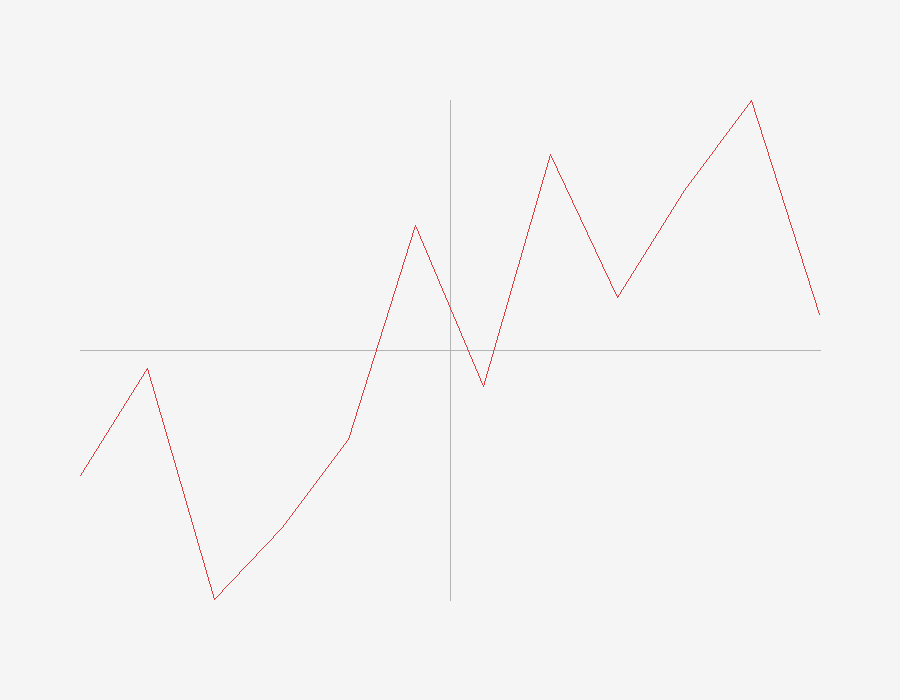
\includegraphics[width=0.8\textwidth]{out_5a_line_graph_dda.png}
    \caption{Line Graph using DDA Algorithm}
\end{figure}

\begin{figure}[H]
    \centering
    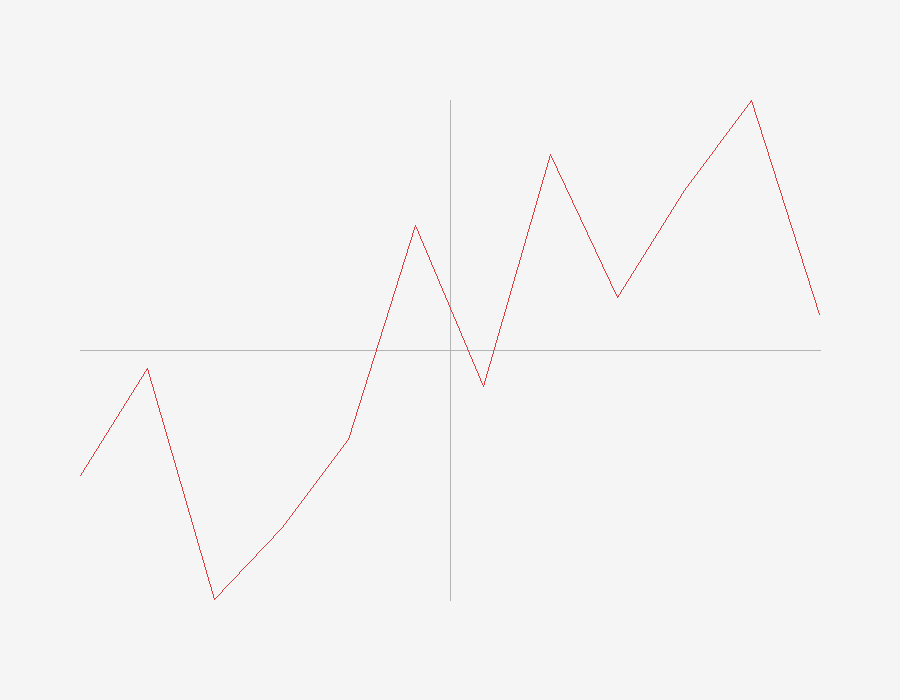
\includegraphics[width=0.8\textwidth]{out_5b_line_graph_bresenham.png}
    \caption{Line Graph using Bresenham Algorithm}
\end{figure}

\newpage
%===========================================
% TASK 6: PIE CHART IMPLEMENTATION
%===========================================
\section{Pie Chart Implementation}

\subsection{Title of Lab Activity}
Implementation of Pie Chart visualization using Midpoint Circle Algorithm and Line Drawing Algorithms.

\subsection{Algorithm}
\begin{enumerate}
    \item Input values for each sector
    \item Calculate total sum and fraction for each sector
    \item Draw outer circle using Midpoint Circle Algorithm
    \item For each sector:
    \begin{itemize}
        \item Calculate start and end angles based on fraction
        \item Generate polygon points along the arc
        \item Fill the sector polygon
        \item Draw boundary lines from center to arc endpoints using line algorithm
    \end{itemize}
\end{enumerate}

\subsection{Source Code}
\begin{lstlisting}[language=Python, caption=Pie Chart Implementation]
import math

def pie_chart(surface, values, rect, colors):
    """
    Draw a pie chart
    values: list of numeric values for each sector
    rect: (x, y, width, height) - bounding rectangle
    colors: list of colors for each sector
    """
    total = sum(values) if values else 0.0
    if total <= 0:
        return

    cx = rect[0] + rect[2] // 2  # Center x
    cy = rect[1] + rect[3] // 2  # Center y
    radius = min(rect[2], rect[3]) // 2 - 4

    # Draw outer circle outline
    midpoint_circle(surface, cx, cy, radius, (150, 150, 150))

    start_angle = 0.0
    two_pi = 2.0 * math.pi

    for idx, val in enumerate(values):
        frac = val / total
        sweep = frac * two_pi
        end_angle = start_angle + sweep
        color = colors[idx % len(colors)]

        # Build polygon points for the sector
        steps = max(12, int(sweep * radius / 6))
        points = [(cx, cy)]
        for k in range(steps + 1):
            theta = start_angle + k * sweep / steps
            x = cx + int(radius * math.cos(theta))
            y = cy + int(radius * math.sin(theta))
            points.append((x, y))

        # Fill sector
        draw.polygon(surface, color, points)

        # Draw boundary lines using Bresenham
        xs = cx + int(radius * math.cos(start_angle))
        ys = cy + int(radius * math.sin(start_angle))
        xe = cx + int(radius * math.cos(end_angle))
        ye = cy + int(radius * math.sin(end_angle))
        bresenham_line(surface, cx, cy, xs, ys, (30, 30, 30))
        bresenham_line(surface, cx, cy, xe, ye, (30, 30, 30))

        start_angle = end_angle
\end{lstlisting}

\subsection{Output}
\begin{figure}[H]
    \centering
    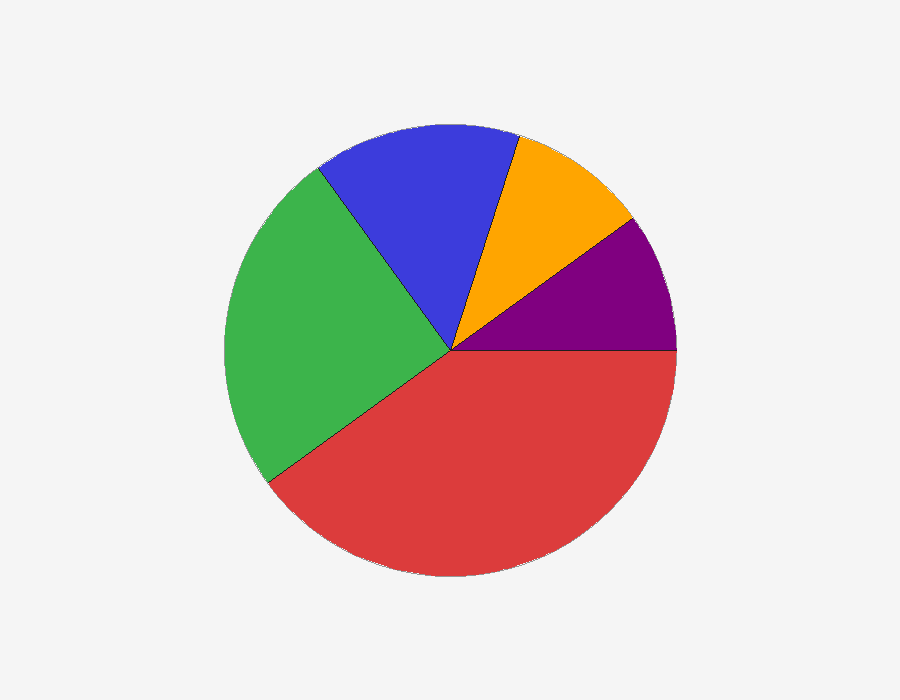
\includegraphics[width=0.8\textwidth]{out_6_pie_chart.png}
    \caption{Pie Chart Implementation Output}
\end{figure}

\newpage
%===========================================
% CONCLUSION
%===========================================
\section{Conclusion}

In this laboratory exercise, we successfully implemented and demonstrated several fundamental computer graphics algorithms:

\begin{enumerate}
    \item \textbf{DDA Line Drawing Algorithm:} We implemented the Digital Differential Analyzer algorithm, which uses incremental floating-point calculations to draw lines. The algorithm is simple to understand and implement, though it requires floating-point arithmetic and rounding operations.
    
    \item \textbf{Bresenham's Line Drawing Algorithm:} We implemented Bresenham's algorithm for both slope conditions ($|m| < 1$ and $|m| \geq 1$). This algorithm uses only integer arithmetic, making it computationally more efficient than DDA. The decision parameter approach eliminates the need for floating-point operations.
    
    \item \textbf{Midpoint Circle Drawing Algorithm:} We implemented the midpoint circle algorithm that exploits 8-way symmetry to efficiently draw circles. The algorithm uses an incremental decision parameter to determine the next pixel position, requiring only integer arithmetic.
    
    \item \textbf{Midpoint Ellipse Drawing Algorithm:} We extended the midpoint concept to ellipses, handling two regions based on the slope of the ellipse. The algorithm uses 4-way symmetry and separate decision parameters for each region.
    
    \item \textbf{Line Graph Implementation:} We demonstrated the practical application of line drawing algorithms by implementing a line graph visualization that can use either DDA or Bresenham algorithm to connect data points.
    
    \item \textbf{Pie Chart Implementation:} We implemented a pie chart that combines the midpoint circle algorithm for the outline and line drawing algorithms for sector boundaries, showing how these fundamental algorithms can be combined for data visualization.
\end{enumerate}

\textbf{Key Learnings:}
\begin{itemize}
    \item Understanding the trade-offs between algorithm simplicity (DDA) and computational efficiency (Bresenham)
    \item The importance of exploiting symmetry in circle and ellipse drawing to reduce computations
    \item How fundamental rasterization algorithms form the building blocks for complex graphics applications
    \item The practical application of these algorithms in data visualization (charts and graphs)
\end{itemize}

\textbf{Observations:}
\begin{itemize}
    \item Bresenham's algorithm produces identical output to DDA but with better performance due to integer-only operations
    \item The midpoint algorithms provide smooth curves by making optimal pixel choices at each step
    \item These scan conversion algorithms are fundamental to all raster graphics systems
\end{itemize}

The laboratory exercise provided hands-on experience with the core algorithms that form the foundation of computer graphics rendering systems.

\end{document}
